\title{x86-64 assembly review}
\date{}
\usepackage{xspace}
\begin{document}
\begin{frame}
    \titlepage
\end{frame}

\usemintedstyle{tango}
\newmintinline{c}{}
\newminted[ccode]{c}{linenos=true,xleftmargin=1cm,beameroverlays,escapeinside=@@,texcomments}
\newminted[ccodeNL]{c}{linenos=false,beameroverlays,escapeinside=@@,texcomments}
\newminted[ccodeS]{c}{linenos=false,fontsize=\small,beameroverlays,escapeinside=@@,texcomments}
\newminted[ccodeT]{c}{linenos=false,fontsize=\scriptsize,beameroverlays,escapeinside=@@,texcomments}
\lstnewenvironment{asmcodeNL}{\lstset{language=myasm,escapeinside=@@,deletekeywords=test}}{}
\lstnewenvironment{asmcodeS}{\lstset{language=myasm,style=small,escapeinside=@@}}{}
\lstnewenvironment{asmcodeT}{\lstset{language=myasm,style=smaller,escapeinside=@@}}{}
\renewcommand{\theFancyVerbLine}{\small\textcolor[rgb]{.25,.25,.25}{\arabic{FancyVerbLine}}}

\usetikzlibrary{calc,positioning}

\begin{frame}
    \titlepage
\end{frame}

\newcommand{\xOF}{\ensuremath{\mathtt{OF}}\xspace}
\newcommand{\xSF}{\ensuremath{\mathtt{SF}}\xspace}
\newcommand{\xCF}{\ensuremath{\mathtt{CF}}\xspace}
\newcommand{\xZF}{\ensuremath{\mathtt{ZF}}\xspace}

\section{assembly: syntax, registers}

\subsection{AT\&T syntax}
\usetikzlibrary{matrix}

\begin{frame}[label=allAttExes]{AT\&T versus Intel syntax by example}
\fontsize{13}{14}\selectfont
{\tt {\keywordstyle movq} \$42, (\%rbx)} \\
\hspace{4cm}{\tt {\keywordstyle mov} QWORD PTR [rbx], 42} \\
{\tt {\keywordstyle subq} \%rax, \%r8} \\
\hspace{4cm}{\tt {\keywordstyle sub} r8, rax} \\
{\tt {\keywordstyle movq} \$42, {100}({\%rbx},{\%rcx,4})} \\
\hspace{4cm}{\tt {\keywordstyle mov} QWORD PTR [{rbx}+{rcx*4}+{100}], 42} \\
{\tt {\keywordstyle jmp} *\%rax} \\
\hspace{4cm} {\tt {\keywordstyle jmp} rax} \\
{\tt {\keywordstyle jmp} *1000(\%rax,\%rbx,8)} \\
\hspace{4cm}{\tt {\keywordstyle jmp} QWORD PTR [RAX+RBX*8+1000]} \\
\end{frame}

\begin{frame}{AT\&T versus Intel syntax (1)}
    \begin{itemize}
    \item AT\&T syntax: \\ {\tt {\keywordstyle movq} \$42, (\%rbx)}
    \item Intel syntax: \\ {\tt {\keywordstyle mov} QWORD PTR [rbx], 42}
    \item effect (pseudo-C): \\ {\tt memory[rbx] <- 42}
    \end{itemize}
\end{frame}

\begin{frame}[fragile,label=att2e1]{AT\&T syntax example (1)}
\lstset{
    language=[x8664gas]Assembler,
    %moredelim=**[is][\color{green!60!black}]{@1*}{*@},
    moredelim=**[is][\btHL<1|handout:0>]{@1*}{*@},
    moredelim=**[is][\btHL<2|handout:0>]{@2*}{*@},
    moredelim={**[is][\btHL<2,4|handout:0>]{@24*}{*@}},
    moredelim=**[is][\btHL<3|handout:0>]{@3*}{*@},
    moredelim=**[is][\btHL<4|handout:0>]{@4*}{*@},
    moredelim=**[is][\btHL<5|handout:0>]{@5*}{*@},
    moredelim=**[is][\btHL<6|handout:0>]{@6*}{*@},
    escapechar=`,
}
\begin{lstlisting}
mov@5*q*@ @3*$42*@, @2*(*@@24*%rbx*@@2*)*@
// memory[rbx] <- 42
\end{lstlisting}
    \begin{itemize}
    \item \myemph<2>{destination last}
    \item {\tt ()}s represent value \myemph<2>{in memory}
    \item \myemph<3>{constants} start with {\tt \$}
    \item \myemph<4>{registers} start with {\tt \%}
    \item {\tt q} (`quad') indicates \myemph<5>{length} (8 bytes)
    \begin{itemize}\item {\tt l}: 4; {\tt w}: 2; {\tt b}: 1
                   \item sometimes can be omitted\end{itemize}
    \end{itemize}
\end{frame}

\begin{frame}{AT\&T versus Intel syntax (2)}
    \begin{itemize}
    \item AT\&T syntax: \\ {\tt \textbf{movq} \$42, \myemph<2>{100}(\myemph<3>{\%rbx},\myemph<4>{\%rcx,4})}
    \item Intel syntax: \\ {\tt \textbf{mov} QWORD PTR [\myemph<3>{rbx}+\myemph<4>{rcx*4}+\myemph<2>{100}], 42}
    \item effect (pseudo-C): \\ {\tt memory[\myemph<3>{rbx} + \myemph<4>{rcx * 4} + \myemph<2>{100}] <- 42}
    \end{itemize}
\end{frame}

\begin{frame}{AT\&T syntax: addressing}
    \begin{itemize}
    \item {\tt 100(\%rbx)}: {\tt memory[rbx + 100]}
    \item {\tt 100(\%rbx,8)}: {\tt memory[rbx * 8 + 100]}
    \item {\tt 100(,\%rbx,8)}: {\tt memory[rbx * 8 + 100]}
    \item {\tt 100(\%rcx,\%rbx,8)}: \\
          \hspace{2cm}{\tt memory[rcx + rbx * 8 + 100]}
    \item {\tt 100}: \\
          \hspace{2cm}{\tt memory[100]}
  \item {\tt 100(\%rbx,\%rcx)}: \\
          \hspace{2cm}{\tt memory[rbx+rcx+100]}
    \end{itemize}
\end{frame}

\begin{frame}[fragile,label=att2e2]{AT\&T versus Intel syntax (3)}
    \begin{itemize}
    \item {\tt r8 $\leftarrow$ r8 - rax}
    \item \begin{tabular}{ll}
        AT\&T syntax: & {\tt {\keywordstyle subq} \%rax, \%r8} \\ 
        Intel syntax: & {\tt {\keywordstyle sub} r8, rax} \\
        \end{tabular}
    \item same for {\tt {\keywordstyle cmp}}
        \begin{itemize}
        \item after {\tt {\keywordstyle cmpq} \%rax, \%r8}, \\
              {\tt jg} jumps if \textbf{\tt \%r8} is greater
          \end{itemize}
    \end{itemize}
\end{frame}

\begin{frame}[fragile,label=attConst]{AT\&T syntax: addresses}
\begin{asmcodeNL}
addq 0x1000, %rax
// Intel syntax: add rax, QWORD PTR [0x1000]
// rax <- rax + memory[0x1000]
addq $0x1000, %rax
// Intel syntax: add rax, 0x1000
// rax <- rax + 0x1000
\end{asmcodeNL}
    \begin{itemize}
        \item no {\tt \$} --- probably memory address 
    \end{itemize}
\end{frame}


\begin{frame}{AT\&T syntax in one slide}
    \begin{itemize}
    \item destination \myemph{last}
    \item {\tt ()} means value \myemph{in memory}
    \item {\tt disp(base, index, scale)} same as \\ {\tt memory[disp + base + index * scale]}
        \begin{itemize}
        \item omit disp (defaults to {\tt 0})
        \item and/or omit base (defaults to {\tt 0})
        \item and/or scale (defualts to {\tt 1})
        \end{itemize}
    \item {\tt \$} means constant
    \item plain number/label means value \myemph{in memory}
    \end{itemize}
\end{frame}

\begin{frame}[fragile,label=compJmpATT]{extra detail: computed jumps}
\begin{asmcodeNL}
jmpq *%rax
// Intel syntax: jmp RAX
    // goto RAX
jmpq *1000(%rax,%rbx,8)
// Intel syntax: jmp QWORD PTR[RAX+RBX*8+1000]
    // read address from memory at RAX + RBX * 8 + 1000
    // go to that address
\end{asmcodeNL}
\end{frame}

\againframe<2>{allAttExes}


\subsection{swap example}  % FIXME: maybe interleave swap example and split AT\&T syntax
\usetikzlibrary{arrows.meta,calc,matrix}
\newcommand{\onSwap}{4}
\newcommand{\onMovA}{5}
\newcommand{\onMovB}{6}
\newcommand{\onMovC}{7}
\newcommand{\onMovD}{8}
\newcommand{\onRet}{9}

\begin{frame}[fragile,label=attSwap]{swap}
\lstset{
    language=myasm,
    style=small,
    moredelim=**[is][\btHL<\onSwap>]{@1}{1@},
    moredelim=**[is][\btHL<\onMovA>]{@2}{2@},
    moredelim=**[is][\btHL<\onMovB>]{@3}{3@},
    moredelim=**[is][\btHL<\onMovC>]{@4}{4@},
    moredelim=**[is][\btHL<\onMovD>]{@5}{5@},
    moredelim=**[is][\btHL<\onRet>]{@6}{6@},
}
\begin{tikzpicture}
\tikzset{
    code box/.style={draw,thick},
    mark read/.style={alt=<#1>{fill=yellow!10}},
    mark read addr/.style={alt=<#1>{fill=blue!10}},
    mark write/.style={alt=<#1>{fill=red!20}},
    mark addr/.style={blue},
    mark value/.style={red},
    >=Latex,
}
\node[code box,label={north:swap (AT\&T syntax)}] (swap att) {
\begin{lstlisting}
// swap(long *rdi,
//      long *rsi)
@1swap1@: 
  @2movq (%rdi), %rax2@
  @3movq (%rsi), %rdx3@
  @4movq %rdx, (%rdi)4@
  @5movq %rax, (%rsi)5@
  @6ret6@
\end{lstlisting}
};
\begin{visibleenv}<2>
\node[code box,alt=<2>{draw=red,very thick},label={north:swap (Intel syntax)},anchor=north west] (swap intel)
    at ([xshift=.5cm]swap att.north east) {
\begin{lstlisting}


swap:
  mov RAX, QWORD PTR [RDI]
  mov RDX, QWORD PTR [RSI]
  mov QWORD PTR [RDI], RDX
  mov QWORD PTR [RSI], RAX
  ret
\end{lstlisting}
};
\end{visibleenv}
\begin{visibleenv}<3>
\node[code box,alt=<3>{draw=red,very thick},label={north:as pseudocode},anchor=north west] (swap pseudo)
    at ([xshift=.5cm]swap att.north east) {
\begin{lstlisting}[language=]


swap:
    RAX <- memory[RDI (arg 1)]
    RDX <- memory[RSI (arg 2)]
    memory[RDI (arg 1)] <- RDX
    memory[RSI (arg 2)] <- RAX
    return
\end{lstlisting}
};
\end{visibleenv}
\begin{visibleenv}<4->
\matrix[tight matrix,
    column 1/.style={nodes={draw=none,text width=1.15cm}},
    column 2/.style={nodes={draw,thick,font=\tt,text width=2.25cm,minimum height=.6cm}},
    row sep=1mm,
    label={north:registers},
    anchor=north west
] (regs) at ([xshift=.5cm]swap att.north east) {
\%rax \& |[alias=rax,mark write=\onMovA,mark read=\onMovD]| \only<1-\onSwap>{???}\only<\onMovA->{0x99999} \\
\%rdx \& |[alias=rdx,mark write=\onMovB,mark read=\onMovC]| \only<1-\onSwap>{???}\only<\onMovB->{0x77777} \\
\%rdi \& |[alias=rdi,mark read addr=\onMovA,mark read addr=\onMovC]| 0x04000 \\
\%rsi \& |[alias=rsi,mark read addr=\onMovB,mark read addr=\onMovD]| 0x04030 \\
\%rsp \& 0xEFFF8 \\
\ldots \& |[draw=none]| \ldots \\
};
\matrix[tight matrix,
    column 1/.style={nodes={draw=none,font=\small\tt,text width=2cm}},
    column 2/.style={nodes={draw,thick,font=\small\tt,text width=2cm,minimum height=.6cm}},
    row 1/.style={nodes={font=\small\bfseries,draw=none}},
    row sep=-0.25mm,
    label={north:memory},
    anchor=north west
] (mem) at ([xshift=1.5cm]regs.north east) {
address \& value \\
0x00000 \& 0xFFFF3\\
0x00008 \& 0x32123 \\
\ldots \& |[draw=none]| \ldots \\
|[alias=starRdiA]| 0x04000 \& |[alias=starRdi,mark read=\onMovA,mark write=\onMovC]| \only<1-\onMovB>{0x99999}\only<\onMovC->{0x77777} \\
0x04008 \& 0x00002 \\
\ldots \& |[draw=none]| \ldots \\
0x04028 \& 0x00090 \\
|[alias=starRsiA]| 0x04030 \& |[alias=starRsi,mark read=\onMovB,mark write=\onMovD]| \only<1-\onMovC>{0x77777}\only<\onMovD->{0x99999} \\
0x04038 \& 0x00078 \\
\ldots \& |[draw=none]| \ldots \\
};
\end{visibleenv}
\begin{visibleenv}<\onMovA>
\draw[->,very thick,mark addr] (rdi.east) -- ++ (.5cm, 0cm) |- ([yshift=-.1cm]starRdiA.west);
\draw[->,very thick,mark value] ([yshift=.1cm]starRdiA.west) -- ++ (-.5cm, 0cm) |- (rax.east);
\end{visibleenv}
\begin{visibleenv}<\onMovB>
\draw[->,very thick,mark addr] (rsi.east) -- ++ (.5cm, 0cm) |- ([yshift=-.1cm]starRsiA.west);
\draw[->,very thick,mark value] ([yshift=.1cm]starRsiA.west) -- ++ (-.5cm, 0cm) |- (rdx.east);
\end{visibleenv}
\begin{visibleenv}<\onMovC>
\draw[->,very thick,mark addr] (rdi.east) -- ++ (.5cm, 0cm) |- ([yshift=-.1cm]starRdiA.west);
\draw[->,very thick,mark value] (rdx.east) -- ++ (1cm, 0cm) |- ([yshift=.1cm]starRdiA.west);
\end{visibleenv}
\begin{visibleenv}<\onMovD>
\draw[->,very thick,mark addr] (rsi.east) -- ++ (.5cm, 0cm) |- ([yshift=-.1cm]starRsiA.west);
\draw[->,very thick,mark value] (rax.east) -- ++ (1cm, 0cm) |- ([yshift=.1cm]starRsiA.west);
\end{visibleenv}
\end{tikzpicture}
\end{frame}


\subsection{x86-64 registers}
\usetikzlibrary{decorations.pathreplacing}

\begin{frame} %{overlapping registers (1)}
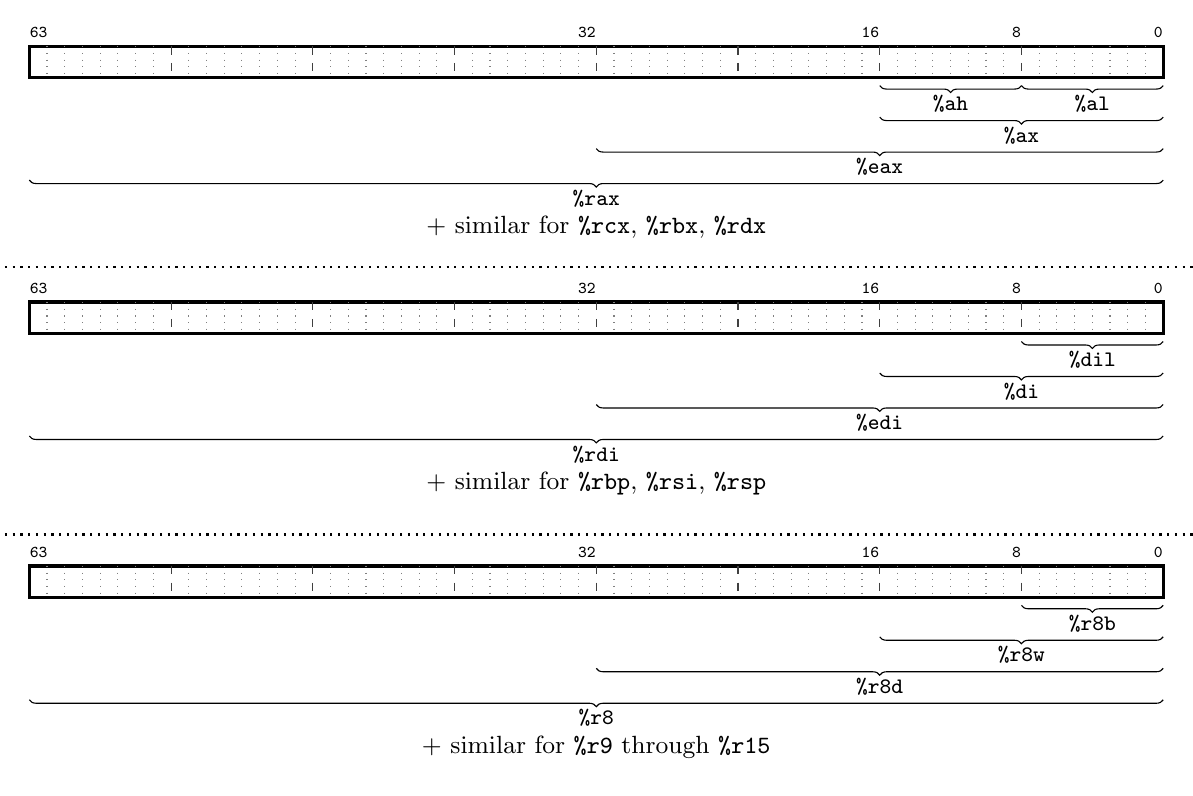
\begin{tikzpicture}
    \tikzset{
        main reg/.style={draw,very thick},
        reg label/.style={font=\fontsize{8.5}{9.5}\tt},
        bit label/.style={font=\fontsize{6}{7}\tt,inner sep=0mm,yshift=1mm},
        reg divider/.style={draw,thin,dashed,black!75},
        reg divider minor/.style={draw,thin,dotted,black!50},
    }
    \draw[overlay,thick,dotted] (-1, -2.8) -- ++(16, 0);
    \draw[overlay,thick,dotted] (-1, -6.2) -- ++(16, 0);
    \providecommand{\regheight}{0.4}
    \begin{scope}[x=0.9cm]
    \node[anchor=south east,bit label] at (16, 0) {0};
    \node[anchor=south east,bit label] at (14, 0) {8};
    \node[anchor=south east,bit label] at (12, 0) {16};
    \node[anchor=south east,bit label] at (8, 0) {32};
    \node[anchor=south west,bit label] at (0, 0) {63};
    \draw[main reg] (0, 0) rectangle (16, -\regheight);
        \foreach \x in {2,4,6,8,10,12,14} {
            \draw[reg divider] (\x, 0) -- ++(0, -\regheight);
        }
        \foreach \x in {0,2,4,6,8,10,12,14} {
            \foreach \xx in {1,2,3,4,5,6,7} {
                \draw[reg divider minor] (\x + \xx * 0.25, 0) -- ++(0, -\regheight);
            };
        }
        \begin{scope}[yshift=-\regheight cm]
        \draw[decorate,decoration={brace,mirror}] (0, -1.3) -- (16, -1.3) node[midway, below, reg label]{ \%rax };
        \draw[decorate,decoration={brace,mirror}] (8, -0.9) -- (16, -0.9) node[midway, below, reg label]{ \%eax };
        \draw[decorate,decoration={brace,mirror}] (12, -0.5) -- (16, -0.5) node[midway, below, reg label]{ \%ax };
        \draw[decorate,decoration={brace,mirror}] (14, -0.1) -- (16, -0.1) node[midway, below, reg label]{ \%al };
        \draw[decorate,decoration={brace,mirror}] (12, -0.1) -- (14, -0.1) node[midway, below, reg label]{ \%ah };
        \end{scope}
            \node[font=\small] at (8, -2.3) { + similar for {\tt \%rcx}, {\tt \%rbx}, {\tt \%rdx} };
    \end{scope}

    \begin{scope}[yshift=-3.25cm]
        \begin{scope}[x=0.9cm]
    \node[anchor=south east,bit label] at (16, 0) {0};
    \node[anchor=south east,bit label] at (14, 0) {8};
    \node[anchor=south east,bit label] at (12, 0) {16};
    \node[anchor=south east,bit label] at (8, 0) {32};
    \node[anchor=south west,bit label] at (0, 0) {63};
    \draw[main reg] (0, 0) rectangle (16, -\regheight);
        \foreach \x in {2,4,6,8,10,12,14} {
            \draw[reg divider] (\x, 0) -- ++(0, -\regheight);
        }
        \foreach \x in {0,2,4,6,8,10,12,14} {
            \foreach \xx in {1,2,3,4,5,6,7} {
                \draw[reg divider minor] (\x + \xx * 0.25, 0) -- ++(0, -\regheight);
            };
        }
        \begin{scope}[yshift=-\regheight cm]
        \draw[decorate,decoration={brace,mirror}] (0, -1.3) -- (16, -1.3) node[midway, below, reg label]{ \%rdi };
        \draw[decorate,decoration={brace,mirror}] (8, -0.9) -- (16, -0.9) node[midway, below, reg label]{ \%edi };
        \draw[decorate,decoration={brace,mirror}] (12, -0.5) -- (16, -0.5) node[midway, below, reg label]{ \%di };
        \draw[decorate,decoration={brace,mirror}] (14, -0.1) -- (16, -0.1) node[midway, below, reg label]{ \%dil };
        \end{scope}
            \node[font=\small] at (8, -2.3) { + similar for {\tt \%rbp}, {\tt \%rsi}, {\tt \%rsp} };
        \end{scope}
    \end{scope}
    \begin{scope}[yshift=-6.6cm]
        \begin{scope}[x=0.9cm]
    \node[anchor=south east,bit label] at (16, 0) {0};
    \node[anchor=south east,bit label] at (14, 0) {8};
    \node[anchor=south east,bit label] at (12, 0) {16};
    \node[anchor=south east,bit label] at (8, 0) {32};
    \node[anchor=south west,bit label] at (0, 0) {63};
    \draw[main reg] (0, 0) rectangle (16, -\regheight);
        \foreach \x in {2,4,6,8,10,12,14} {
            \draw[reg divider] (\x, 0) -- ++(0, -\regheight);
        }
        \foreach \x in {0,2,4,6,8,10,12,14} {
            \foreach \xx in {1,2,3,4,5,6,7} {
                \draw[reg divider minor] (\x + \xx * 0.25, 0) -- ++(0, -\regheight);
            };
        }
        \begin{scope}[yshift=-\regheight cm]
        \draw[decorate,decoration={brace,mirror}] (0, -1.3) -- (16, -1.3) node[midway, below, reg label]{ \%r8 };
        \draw[decorate,decoration={brace,mirror}] (8, -0.9) -- (16, -0.9) node[midway, below, reg label]{ \%r8d };
        \draw[decorate,decoration={brace,mirror}] (12, -0.5) -- (16, -0.5) node[midway, below, reg label]{ \%r8w };
        \draw[decorate,decoration={brace,mirror}] (14, -0.1) -- (16, -0.1) node[midway, below, reg label]{ \%r8b };
        \end{scope}
            \node[font=\small] at (8, -2.3) { + similar for {\tt \%r9} through {\tt \%r15} };
        \end{scope}
    \end{scope}

\end{tikzpicture}
\end{frame}




\begin{frame}[fragile,label=overlapEx]{overlapping registers (1)}
    \begin{itemize}
    \item setting 32-bit registers --- clears corresponding 64-bit register
\begin{asmcodeNL}
movq $0xFFFFFFFFFFFFFFFF, %rax
movl $0x1, %eax
\end{asmcodeNL}
        \item \%rax is {\tt 0x1} ({\small not {\tt 0xFFFFFFFF00000001}})
    \end{itemize}
\end{frame}
\begin{frame}[fragile,label=overlapEx2]{overlapping registers (2)}
\begin{itemize}
    \item setting 8/16-bit registers: don't clear 64-bit register
\begin{asmcodeNL}
movq $0xFFFFFFFFFFFFFFFF, %rax
movb $0x1, %al
\end{asmcodeNL}
    \item \%rax is {\tt 0xFFFFFFFFFFFFFF01}
\end{itemize}
\end{frame}



\subsection{on labels}
\begin{frame}[fragile,label=labels0]{labels (1)}
    \begin{itemize}
    \item labels represent \myemph{addresses}
    \end{itemize}
\end{frame}

\begin{frame}[fragile,label=labels1]{labels (2)}
\begin{asmcodeS}
    addq string, %rax
    // intel syntax: add rax, QWORD PTR [label]
    // rax <- rax + memory[address of "a string"]
    addq $string, %rax
    // intel syntax: add rax, OFFSET label
    // rax <- rax + address of "a string"
string:  .ascii "a string"
\end{asmcodeS}
\begin{itemize}
    \item {\tt addq label}: read value at the address
    \item {\tt addq \$label}: use address as an integer constant
\end{itemize}
\end{frame}

\begin{frame}<0>[fragile,label=labels2]{labels (3)}
\begin{asmcodeS}
loop:    
    subq $1, %rax
    cmpq $0, %rax
    jge loop
\end{asmcodeS}
\begin{itemize}
    \item puts \myemph{address of subq} {\small (or equivalent)} in {\keywordstyle jge} 
    \item recall: symbol table entry and relocation in object file
\end{itemize}
\end{frame}



\subsection{AT\&T syntax exercise}
\begin{frame}[fragile,label=attExercise]{exericse}
\begin{lstlisting}[language=myasm,style=smaller]
hello:
    .string "Hello, World!" ; nul-terminated string
example:
    movb hello+1, %bl
    subb $1, %bl
    movb %bl, hello
    movq $hello, %rdi
    ; int puts(const char *s [%rdi])
    callq puts
    ret
\end{lstlisting}
What is the the argument to puts, \%rdi?

\small
\begin{tabular}{ll}
A. a pointer to `Hello, World!' & B. a pointer to `dello, World!' \\
C. a pointer to `Hdllo, World!' & D. a pointer to `fello, World!' \\
E. a pointer to `Jello, World!' & F. a pointer to a different string \\
\end{tabular}
\begin{tabular}{l}
G. an integer constructed from the ASCII for `Hello, W' (puts probably crashes) \\
H. an integer constructed from the ASCII for `Jello, W' (puts probably crashes) \\
I. an integer constructed from the ASCII for a different string (puts probably crashes) \\
\end{tabular}
\end{frame}

\iftoggle{heldback}{}{\usetikzlibrary{arrows.meta,matrix}

\begin{frame}[fragile,label=attExerciseSoln]{exercise (explanation)}
\begin{lstlisting}[language=myasm,style=smaller,morekeywords=subb,deletekeywords=bl]
hello:
  .string "Hello, World!" ; nul-terminated string
example:
  movb hello+1, %bl
    // hello = address of 'H' in string, hello+1 = addr of 'e', ...
    // %bl becomes 'e'
  subb $1, %bl
    // %bl becomes 'd'
  movb %bl, hello
    // move 'd' to where 'H' is stored; string now "dello, World!"
  movq $hello, %rdi
    // move address of (first char in) the string "dello, World"
  ; int puts(const char *s [%rdi])
  callq puts
  ret
\end{lstlisting}
\begin{tikzpicture}
    \matrix[tight matrix,nodes={font=\small\tt,text width=.5cm}] (string text) {
        |[alt=<2>{fill=red!10}]| \alt<2->{d}{H} \& e \& l \& l \& o \& \ldots \\
};
\node[align=center,font=\small\tt,anchor=north] (hello label) at ([yshift=-.2cm]string text.south west) {
    {hello} \\
    {0x123456}
};
    \draw[very thick,-Latex] (hello label.north) -- (string text-1-1.south);
\node[align=center,font=\small\tt,anchor=north] (hello1 label) at ([xshift=3cm,yshift=-.2cm]string text.south west) {
    {hello + 1} \\
    {0x123457}
};
    \draw[very thick,-Latex] (hello1 label.north) -- (string text-1-2.south);
\end{tikzpicture}
\end{frame}
}

\subsection{LEA}

\begin{frame}[fragile,label=LEA]{on LEA}
    \begin{itemize}
        \item LEA = \textbf{L}oad \textbf{E}ffective \textbf{A}ddress
        \begin{itemize}
            \item effective address = computed address for memory access
        \end{itemize}
    \item syntax looks like a \textbf{mov} from memory, but\ldots
    \item \myemph{skips the memory access} --- just uses the address
        \begin{itemize}
            \item (sort of like {\tt \&} operator in C?)
        \end{itemize}
    \item {}\lstinline|leaq 4(%rax), %rax| $\approx$ \lstinline|addq $4, %rax|
    \item<2-> ``address of memory[rax + 4]'' = rax + 4
    \end{itemize}
\end{frame}

\begin{frame}[fragile,label=LEATricks]{LEA tricks}
    \begin{itemize}
    \item {}\lstinline|leaq (%rax,%rax,4), %rax|
    \item rax $\leftarrow$ rax $\times$ 5
    \item rax $\leftarrow$ {\tt address-of(memory[rax + rax * 4])}
    \vspace{.5cm}
            \hrule
    \vspace{.5cm}
    \item {}\lstinline|leaq (%rbx,%rcx), %rdx|
    \item rdx $\leftarrow$ rbx $+$ rcx
    \item rdx $\leftarrow${\tt address-of(memory[rbx + rcx])}
    \end{itemize}
\end{frame}



\subsubsection{exercise}

\begin{frame}[fragile,label=usingLEATricks]{exercise: what is this function?}
\begin{asmcodeNL}
mystery:
    leal 0(,%rdi,8), %eax
    subl %edi, %eax
    ret
\end{asmcodeNL}
\begin{ccodeNL}
int mystery(int arg) { return ...; }
\end{ccodeNL}
\begin{tabular}{ll}
A. {\tt arg * 9}  & D. {\tt -arg * 7} \\
B. {\tt -arg * 9} & E. \maybeEmph<2>{none of these} \\
C. {\tt arg * 8}  & F. it has a different prototype \\
\end{tabular}
\end{frame}


\subsection{review: calling convention}
\begin{frame}{Linux x86-64 calling convention}
    \begin{itemize}
    \item \myemph{registers} for first 6 arguments:
    \begin{itemize}
    \item {\tt \%rdi} (or {\tt \%edi} or {\tt \%di}, etc.), then
    \item {\tt \%rsi} (or {\tt \%esi} or {\tt \%si}, etc.), then
    \item {\tt \%rdx} (or {\tt \%edx} or {\tt \%dx}, etc.), then
    \item {\tt \%rcx} (or {\tt \%ecx} or {\tt \%cx}, etc.), then
    \item {\tt \%r8} (or {\tt \%r8d} or {\tt \%r8w}, etc.), then
    \item {\tt \%r9} (or {\tt \%r9d} or {\tt \%r9w}, etc.)
    \end{itemize}
    \item rest on stack
    \item return value in {\tt \%rax}
    \item don't memorize: Figure 3.28 in book
    \end{itemize}
\end{frame}

% FIXME: %rip?

\begin{frame}[fragile,label=x8664CCExample]{x86-64 calling convention example}
\begin{ccodeNL*}{fontsize=\small}
int foo(int x, int y, int z) { return 42; }
...
    foo(1, 2, 3);
...
\end{ccodeNL*}
\hrule
\begin{asmcodeS}
...
    // foo(1, 2, 3)
    movl $1, %edi
    movl $2, %esi
    movl $3, %edx
    call foo  // call pushes address of next instruction
              // then jumps to foo
...
foo: 
    movl $42, %eax
    ret
\end{asmcodeS}
\end{frame}

\begin{frame}[fragile,label=stackFrame]{call/ret}
\begin{itemize}
\item call:
    \begin{itemize}
    \item push address of \myemph{next instruction} on the stack
    \end{itemize}
\item ret:
    \begin{itemize}
    \item pop address from stack; jump
    \end{itemize}
\end{itemize}
\end{frame}

\begin{frame}[fragile,label=calleeSaved]{callee-saved registers}
    \begin{itemize}
    \item functions \myemph{must preserve} these
    \vspace{.5cm}
    \item {\tt \%rsp} (stack pointer), {\tt \%rbx}, {\tt \%rbp} (frame pointer, maybe)
    \item {\tt \%r12-\%r15}
    \end{itemize}
\end{frame}

\begin{frame}[fragile,label=callerCallee]{caller/callee-saved}
\lstset{style=small}
\begin{lstlisting}
foo:
    pushq %r12 // r12 is callee-saved
    ... use r12 ...
    popq %r12
    ret

...
other_function:
    ...
    pushq %r11 // r11 is caller-saved
    callq foo
    popq %r11
\end{lstlisting}
\end{frame}



\subsection{what we won't cover}

\begin{frame}{selected things we won't cover (today)}
    \begin{itemize}
        \item floating point; vector operations (multiple values at once)
            \begin{itemize}
            \item special registers: \%xmm0 through \%xmm15
            \end{itemize}
        \item segmentation (special registers: \%ds, \%fs, \%gs, \ldots)
        \item lots and lots of instructions
    \end{itemize}
\end{frame}


\section{assembly: control flow}

\subsection{condition codes: briefly}
\begin{frame}[fragile,label=x86IfExample]{conditionals in x86 assembly}
\begin{lstlisting}[language=C++]
    if (rax != 0)
        foo();
\end{lstlisting}
\hrule
\begin{lstlisting}[language=myasm]
    cmpq $0, %rax
    // ***
    je skip_call_foo
    call foo
skip_call_foo:
\end{lstlisting}
\hrule
\begin{itemize}
\item how does \texttt{je} know the result of the comparison?
\item what happens if we add extra instructions at the \texttt{***}?
\end{itemize}
\end{frame}

\begin{frame}{condition codes}
\begin{itemize}
\item x86 has \myemph{condition codes}
\item special registers set by (almost) all arithmetic instructions
    \begin{itemize}
    \item addq, subq, imulq, etc.
    \end{itemize}
\item store info about \myemph{last arithmetic result}
    \begin{itemize}
    \item was it zero? was it negative? etc.
    \end{itemize}
\end{itemize}
\end{frame}

\begin{frame}{condition codes and jumps}
\begin{itemize}
\item {\keywordstyle jg}, {\keywordstyle jle}, etc. read condition codes
\item named based on interpreting \myemph{result of subtraction}
    \begin{itemize}
    \item alternate view: comparing result to 0
    \end{itemize}
\item 0: equal; negative: less than; positive: greater than
\end{itemize}
\end{frame}




\subsection{condition codes: detail}
\begin{frame}<1-3>[fragile,label=exShort]{condition codes: closer look}
\begin{itemize}
    \item \xZF (``zero flag'') --- was result zero? (sub/cmp: equal)
        \begin{itemize}
        \item e.g. JE (jump if equal) checks for ZF = 1
        \end{itemize}
    \item \xSF (``sign flag'') --- was result negative? (sub/cmp: less)
        \begin{itemize}
        \item e.g. JL (jump if less than) checks for SF = 1 (plus extra case for overflow)
        \item e.g. JLE checks for SF = 1 or ZF = 1 (plus overflow)
        \end{itemize}
    \item<2-> \xOF (``overflow flag'') --- did computation overflow (as signed)?
        \begin{itemize}
        \item<2-> we won't test on this/use it in later assignments
        \item<2-> signed conditional jumps: JL, JLE, JG, JGE, \ldots
        \end{itemize}
    \item<2-> \xCF (``carry flag'') --- did computation overflow (as unsigned)?
        \begin{itemize}
        \item<2-> we won't test on this/use it in later assignments
        \item<2-> unsigned conditional jumps: JB, JBE, JA, JAE, \ldots
        \end{itemize}
    \item \only<1>{(and some more, e.g. to handle overflow)}\only<2->{(and one more)}
\end{itemize}
\end{frame}

\begin{frame}[fragile,label=ccGdbEx]{condition codes (and other flags) in GDB}
\begin{lstlisting}[
    language={},
    moredelim={**[is][\btHL]{@*}{*@}},
]
(gdb) info registers
rax            0x0                 0
rbx            0x555555555150      93824992235856
rcx            0x555555555150      93824992235856
...
rip            0x55555555513a      0x55555555513a <main+17>
@*eflags*@         0x246               [ @*PF ZF IF*@ ]
cs             0x33                51
ss             0x2b                43
...
\end{lstlisting}
ZF = 1 (listed); SF, OF, CF clear \\
some other flags that you can lookup (PF, IF) also shown
\end{frame}


\subsection{condition code example}
\begin{frame}[fragile,label=ccEx1]{condition codes example (1)}
\begin{lstlisting}
  movq $-10, %rax
  movq $20, %rbx
  subq %rax, %rbx // %rbx - %rax = 30
    // result > 0: %rbx was > %rax
  jle foo // not taken; 30 > 0
\end{lstlisting}
\only<2->{30: SF = 0 (not negative), ZF = 0 (not zero)}
\end{frame}

  %FIXME: loop reference?

\begin{frame}[fragile,label=ccEx1b]{condition codes example (1b)}
\begin{lstlisting}[style=small]
  movq $-10, %rax
  movq $20, %rbx
  subq %rax, %rbx // %rbx - %rax = 30 
  jle foo // not taken; 30 > 0
\end{lstlisting}
30: SF = 0 (not negative), ZF = 0 (not zero)
\hrule
\begin{lstlisting}[style=small]
  movq $20, %rax
  movq $20, %rbx
  subq %rax, %rbx // %rbx - %rax = 0
  jle foo // taken; 0 <= 0
\end{lstlisting}
0: SF = 0 (not negative), ZF = 1 (zero)
\hrule
\begin{lstlisting}[style=small]
  movq $0, %rax
  movq $-10, %rbx
  subq %rax, %rbx // %rbx - %rax = -10
  jle foo // taken; -10 <= 0
\end{lstlisting}
-10: SF = 1 (negative), ZF = 0 (not zero)
\end{frame}



\subsection{cmp}
\begin{frame}{condition codes and cmpq}
\begin{itemize}
\item ``\myemph{last arithmetic result}''???
\item then what is cmp, etc.?
\item \texttt{cmp} does \myemph{subtraction} (but doesn't store result)
\vspace{.5cm}
\item similar \texttt{test} does bitwise-and
\item {\tt {\keywordstyle testq} \%rax, \%rax} --- result is \%rax
\end{itemize}
\end{frame}




\subsection{what sets condition codes}
\begin{frame}[fragile,label=setCC]{what sets condition codes}
\begin{itemize}
\item \textit{most} instructions that compute something \myemph{set condition codes}
\item some instructions \myemph{only} set condition codes:
    \begin{itemize}
    \item {\keywordstyle cmp} $\sim$ {\keywordstyle sub}
    \item {\keywordstyle test} $\sim$ {\keywordstyle and} (bitwise and --- later)
    \item \lstinline|testq %rax, %rax| --- result is \%rax
    \end{itemize}
\item some instructions don't change condition codes:
    \begin{itemize}
    \item {\keywordstyle lea}, {\keywordstyle mov}
    \item control flow: {\keywordstyle jmp}, {\keywordstyle call}, {\keywordstyle ret}, {\keywordstyle jle}, etc.
    \end{itemize}
\item how do you know? --- check processor's manual
\end{itemize}
\end{frame}



\subsection{example with cmp}


\begin{frame}<1-2>[fragile,label=ccEx2]{condition codes example (2)}
\begin{lstlisting}
movq $-10, %rax  // rax <- (-10)
movq $20, %rbx   // rbx <- 20
cmpq %rax, %rbx  // set cond codes w/ rbx - rax
jle foo // not taken; %rbx - %rax > 0
\end{lstlisting}
\only<2->{\%rbx - \%rax = 30: SF = 0 (not negative), ZF = 0 (not zero)}
\end{frame}




\subsection{omitting cmps}

\begin{frame}[fragile,label=omitCmp]{omitting the cmp}
\begin{lstlisting}[language=myasm,style=small]
    movq $99, %r12          // x (r12) <- 99
start_loop:
    call foo                // foo()
    subq $1, %r12           // x (r12) <- x - 1
    cmpq $0, %r12  
    // compute x (r12) - 0 + set cond. codes 
    jge  start_loop         // r12 >= 0?
                            // or result >= 0?
\end{lstlisting}
\hrule
\begin{lstlisting}[language=myasm,style=small]
    movq $99, %r12          // x (r12) <- 99
start_loop:
    call foo                // foo()
    subq $1, %r12           // x (r12) <- x - 1
    jge  start_loop         // new r12 >= 0?
\end{lstlisting}
\end{frame}


\subsection{exercise: what possible? (1)}
\begin{frame}[fragile,label=ccExer]{condition code exercise}
\begin{lstlisting}[language=myasm]
movq %rcx, %rdx
subq $1, %rdx
addq %rdx, %rcx
\end{lstlisting}
\sout<2->{Assuming no overflow,} possible values of SF, ZF?
\begin{tabular}{l}
A. SF = 0, ZF = 0 \\
B. SF = 1, ZF = 0 \\
C. SF = 0, ZF = 1 \\
D. SF = 1, ZF = 1 \\
\end{tabular}
\end{frame}


\subsection{exercise: how used?}
\begin{frame}{exercise}
\begin{itemize}
\item (ignoring overflow) \texttt{jge} is taken (jumps to target) when
    \begin{itemize}
    \item A. ZF = 1
    \item B. SF = 1
    \item C. SF = 1 and ZF = 0
    \item D. SF = 1 or ZF = 1
    \item E. SF = 0
    \item F. something else
    \end{itemize}
\end{itemize}
\end{frame}



\section{C to assembly}

\subsection{if to assembly}

% FIXME: hilight corresponding regions
\begin{frame}[fragile,label=ifToAsm1]{if-to-assembly (1)}
\begin{ccodeNL}
if (b >= 42) {
    a += 10;
} else {
    a *= b;
}
\end{ccodeNL}
\begin{visibleenv}<2>
\hrule
\begin{ccodeNL}
            if (b < 42) goto after_then;
            a += 10;
            goto after_else;
after_then: a *= b;
after_else:
\end{ccodeNL}
\end{visibleenv}
\end{frame}

\begin{frame}[fragile,label=ifToAsm2]{if-to-assembly (2)}
\begin{ccodeNL}
if (b >= 42) {
    a += 10;
} else {
    a *= b;
}
\end{ccodeNL}
\hrule
\begin{lstlisting}[language=myasm,style=small]
// a is in %rax, b is in %rbx
    cmpq $42, %rbx   // computes rbx - 42 to 0
                     // i.e compare rbx to 42
    jl after_then    // jump if rbx - 42 < 0 
                     // AKA rbx < 42
    addq $10, %rax   // a += 10
    jmp after_else
after_then:
    imulq %rbx, %rax // rax = rax * rbx
after_else:
\end{lstlisting}
\end{frame}



% POSSIBLY SIMPLIFY?
\subsubsection{exercise}

\begin{frame}[fragile,label=ifToAsmEx]{exercise}
\begin{lstlisting}[language=myasm,style=smaller]
    subq %rax, %rbx
    addq %rbx, %rcx
    je after
    addq %rax, %rcx
after:
\end{lstlisting}
This is equivalent to what C code? {\scriptsize (rax = var. assigned to register \%rax, etc.)}

\begin{tikzpicture}
\tikzset{
    code box/.style={draw,minimum width=6.5cm,minimum height=2cm,font=\fontsize{9}{10}\selectfont,align=left}
}
\node[code box] (code1) at (0,0) {
\begin{lstlisting}[language=C,style=smaller]
rbx -= rax;
rcx += rbx;
if (rcx == 0) {
    rcx += rax;
}
\end{lstlisting}
};
\node[code box] (code2) at (7.5,0) {
\begin{lstlisting}[language=C,style=smaller]
rbx -= rax;
rcx += rbx;
if (rbx == rcx) {
    rcx += rax;
}
\end{lstlisting}
};
\node[code box] (code3) at (0,-3) {
\begin{lstlisting}[language=C,style=smaller]
rbx -= rax;
rcx += rbx;
if (rbx + rcx == 0) {
    rcx += rax;
}
\end{lstlisting}
};
\node[code box] (code4) at (7.5,-3) {
\begin{lstlisting}[language=C,style=smaller]
rcx += (rbx - rax);
if (rcx == (rbx - rax)) {
    rcx += rax;
}
\end{lstlisting}
};
\foreach \x/\lbl in {1/A,2/B,3/C,4/D} {
    \node[draw,thick,circle,anchor=center,fill=white]  at (code\x.north west) {\lbl};
}
\end{tikzpicture}
\end{frame}

\iftoggle{heldback}{}{\usetikzlibrary{arrows.meta,shapes}

\begin{frame}[fragile,label=ifToAsmEx]{exercise}
\begin{lstlisting}[language=myasm,style=smaller]
    subq %rax, %rbx
    addq %rbx, %rcx
    je after
    addq %rax, %rcx
after:
\end{lstlisting}
Same as which of these C snippets? {\scriptsize (rax = var. assigned to register \%rax, etc.)}

\begin{tikzpicture}
\tikzset{
    code box/.style={draw,minimum width=6.5cm,minimum height=2cm,font=\fontsize{9}{10}\selectfont,align=left}
}
\node[code box] (code1) at (0,0) {
\begin{lstlisting}[language=C,style=smaller]
rbx -= rax;
rcx += rbx;
if (rcx == 0) {
    rcx += rax;
}
\end{lstlisting}
};
    \node [red,font=\large\bfseries] (not mark) at ([yshift=-1.2cm,xshift=.2cm]code1.north) {!};
\node[code box] (code2) at (7.5,0) {
\begin{lstlisting}[language=C,style=smaller]
rbx -= rax;
rcx += rbx;
if (rbx == rcx) {
    rcx += rax;
}
\end{lstlisting}
};
\node[code box] (code3) at (0,-3) {
\begin{lstlisting}[language=C,style=smaller]
rbx -= rax;
rcx += rbx;
if (rbx + rcx == 0) {
    rcx += rax;
}
\end{lstlisting}
};
\node[code box] (code4) at (7.5,-3) {
\begin{lstlisting}[language=C,style=smaller]
rcx += (rbx - rax);
if (rcx == (rbx - rax)) {
    rcx += rax;
}
\end{lstlisting}
};
    \draw[Latex-, red, very thick,overlay] (not mark.north east) -- ++(2cm, 3cm) node[above right,fill=white] {
        would be correct with flipped compare
    };
\foreach \x/\lbl in {1/A,2/B,3/C,4/D} {
    \node[draw,thick,circle,anchor=center,fill=white] (mark \lbl) at (code\x.north west) {\lbl};
    \node[draw,cross out,red,ultra thick] at (mark \lbl) {};
}
\end{tikzpicture}
\end{frame}
}

\subsection{loops to assembly}

\begin{frame}[fragile,label=loop3]{while-to-assembly (1)}
\begin{ccodeS}
while (x >= 0) {
    foo()
    x--;
} 
\end{ccodeS}
\hrule
\begin{visibleenv}<2->
\begin{ccodeS}
start_loop:
    if (x < 0) goto end_loop;
    foo()
    x--;
    goto start_loop:
end_loop:
\end{ccodeS}
\end{visibleenv}
\end{frame}

\begin{frame}[fragile,label=loop4]{while-to-assembly (2)}
\begin{ccodeS}
start_loop:
    if (x < 0) goto end_loop;
    foo()
    x--;
    goto start_loop:
end_loop:
\end{ccodeS}
\hrule
\begin{lstlisting}[language=myasm,style=small]
start_loop:
    cmpq $0, %r12 
    jl end_loop // jump if r12 - 0 < 0
    call foo
    subq $1, %r12
    jmp start_loop 
\end{lstlisting}
\end{frame}



\subsection{exercise: while to assembly}

\begin{frame}[fragile,label=whileEx]{while exercise}
\begin{ccodeNL}
while (b < 10) { foo(); b += 1; }
\end{ccodeNL}
Assume b is in \myemph{callee-saved} register \%rbx.
Which are correct assembly translations?
\begin{tikzpicture}
%\tikzset{every node/.style={inner sep=0cm,outer sep=0cm}}
\node (vA) {
\begin{asmcodeT}
// version A
start_loop:
  call foo
  addq $1, %rbx
  cmpq $10, %rbx
  jl start_loop
\end{asmcodeT}
};
\node[anchor=north west] (vB) at ([xshift=1cm]vA.north east) {
\begin{asmcodeT}
// version B
start_loop:
  cmpq $10, %rbx
  jge end_loop
  call foo
  addq $1, %rbx
  jmp start_loop
end_loop:
\end{asmcodeT}
};
\node[anchor=north west] (vC) at ([xshift=1cm]vB.north east) {
\begin{asmcodeT}
// version C
start_loop:
  movq $10, %rax
  subq %rbx, %rax
  jge end_loop
  call foo
  addq $1, %rbx
  jmp start_loop
end_loop:
\end{asmcodeT}
};
\begin{comment}
%\node[anchor=north west] (vD) at ([xshift=1cm]vC.north east) {
%\begin{asmcodeT}
%// version D
%  cmpq $10, %rbx
%  jge end_loop
%  movq $10, %r12
%  subq %rbx, %r12
%start_loop:
%  call foo
%  decq %r12
%  jge start_loop
%end_loop:
%  movq $10, %rbx
%\end{asmcodeT}
%};
\end{comment}
    \draw[thick] ([xshift=.5cm]vA.north east) -- ([xshift=.5cm]vA.south east);
    \draw[thick] ([xshift=.5cm]vB.north east) -- ([xshift=.5cm]vB.south east);
\end{tikzpicture}
\end{frame}

\begin{frame}[fragile,label=whileExWork]{while exercise: translating?}
\begin{ccodeNL}
while (b < 10) {
    foo();
    b += 1;
}
\end{ccodeNL}
\hrule
\begin{visibleenv}<2>
\begin{ccodeNL}
start_loop: if (b < 10) goto end_loop;
            foo();
            b += 1;
            goto start_loop;
end_loop:
\end{ccodeNL}
\end{visibleenv}
\end{frame}


\subsection{while to assembly: opt levels}

\begin{frame}[fragile,label=loopAsmEx]{while --- levels of optimization}
\begin{ccodeNL*}{fontsize=\small}
while (b < 10) { foo(); b += 1; }
\end{ccodeNL*}
\lstset{
    language=myasm,
    style=smaller,
    escapechar=`,
    morekeywords=decq,
}
\begin{tabular}{l|l|l}
\begin{minipage}{4.7cm}
\begin{visibleenv}<1->
\begin{lstlisting}
start_loop:
  cmpq $10, %rbx
  jge end_loop
  call foo
  addq $1, %rbx
  jmp start_loop
end_loop:
    ...
    ...
    ...
    ...
\end{lstlisting}
\end{visibleenv}
\end{minipage}
&
\begin{minipage}{4.5cm}
\begin{visibleenv}<2->
\begin{lstlisting}
  cmpq $10, %rbx
  jge end_loop
start_loop:
  call foo
  addq $1, %rbx
  cmpq $10, %rbx
  jne start_loop
end_loop:
    ...
    ...
    ...
\end{lstlisting}
\end{visibleenv}
\end{minipage}
&
\begin{minipage}{4.7cm}
\begin{visibleenv}<3->
\begin{lstlisting}
  cmpq $10, %rbx
  jge end_loop
  movq $10, %rax
  subq %rbx, %rax
  movq %rax, %rbx
start_loop:
  call foo
  decq %rbx
  jne start_loop
  movq $10, %rbx
end_loop:
\end{lstlisting}
\end{visibleenv}
\end{minipage}
\end{tabular}
\end{frame}



\subsection{switch statements}

\usetikzlibrary{arrows.meta,decorations.pathreplacing,matrix}

\begin{frame}[fragile,label=compSw1]{compiling switches (1)}
\begin{ccodeNL*}{fontsize=\small}
switch (a) {
    case 1: ...; break;   
    case 2: ...; break;
    ...
    default: ...
}
\end{ccodeNL*}
\lstset{
    language=myasm,
    style=smaller,
    escapechar=`,
    morekeywords=decq,
}
\begin{lstlisting}
    // same as if statement?
    cmpq $1, %rax
    je code_for_1
    cmpq $2, %rax
    je code_for_2
    cmpq $3, %rax
    je code_for_3
    ...
    jmp code_for_default
\end{lstlisting}
\end{frame}

\begin{frame}[fragile,label=compSw2]{compiling switches (2)}
\begin{ccodeNL*}{fontsize=\small}
switch (a) {
    case 1: ...; break;
    case 2: ...; break;
    ...
    case 100: ...; break;
    default: ...
}
\end{ccodeNL*}
\lstset{
    language=myasm,
    style=smaller,
    escapechar=`,
    morekeywords=decq,
}
\begin{lstlisting}
    // binary search
    cmpq $50, %rax
    jl code_for_less_than_50
    cmpq $75, %rax
    jl code_for_50_to_75
    ...
code_for_less_than_50:
    cmpq $25, %rax
    jl less_than_25_cases
    ...
\end{lstlisting}
\end{frame}

\begin{frame}[fragile,label=compSw3]{compiling switches (3a)}
\begin{ccodeNL*}{fontsize=\small}
switch (a) {
    case 1: ...; break;
    case 2: ...; break;
    ...
    case 100: ...; break;
    default: ...
}
\end{ccodeNL*}
\lstset{
    language=myasm,
    style=smaller,
    escapechar=`,
    morekeywords={decq,.quad}
}
\begin{tabular}{l@{\hspace{1cm}}l}
{\begin{lstlisting}
// jump table
cmpq $100, %rax
jg code_for_default
cmpq $1, %rax
jl code_for_default
jmp *table - 8(,%rax,8)
\end{lstlisting}
}
    &
{\begin{lstlisting}
table:
  // not instructions
  // .quad = 64-bit (4 x 16) constant
  .quad code_for_1
  .quad code_for_2
  .quad code_for_3
  .quad code_for_4
    ...
\end{lstlisting}
} 
\end{tabular}
\end{frame}

% FIXME: visualization here
\begin{frame}[fragile,label=compSw3b]{compiling switches (3b)}
\begin{tikzpicture}
\tikzset{
    hilite table/.style={alt=<2>{fill=red!10}},
}
\node[font=\tt] (asm) {
    jmp *table-8(,\%rax,8)
};
\node[anchor=north west,draw,font=\small,align=left] at ([xshift=1cm]asm.north east) {
    \myemph<3>{suppose RAX = 2}, \\ \myemph<2>{\texttt{table} located at 0x12500} 
};
\begin{visibleenv}<2->
\matrix[tight matrix,
    nodes={text width=2.3cm},
    column 1/.style={nodes={
        draw=none,text width=3cm,align=right,font=\fontsize{9}{10}\selectfont\tt\color{blue!70!black},
    }},
    column 2/.style={nodes={draw=none,font=\tt\small}},
    column 3/.style={nodes={font=\tt}},
    anchor=north west
] at (asm.south west){
    \& \normalfont\bfseries address \& |[draw=none]|\normalfont\bfseries value \\
    ~ \& \ldots \& |[draw=none]|\ldots\\
    ~ \& 0x124F8 \& |[draw=none]| \ldots \\
    table \& 0x12500 \& |[hilite table,alias=table top]| 0x13008 \\
    table + 0x08 \& 0x12508 \& |[hilite table,alias=table target]| 0x130A0 \\
    table + 0x10 \& 0x12510 \& |[hilite table]| 0x130C8 \\
    table + 0x18 \& 0x12518 \& |[hilite table]| 0x13110 \\
    ~ \& \ldots \& |[draw=none,alias=table bottom]|\ldots\\
    ~ \\
    ~ \& \ldots \& |[draw=none]|\ldots\\
    code\_for\_1 \& 0x13008 \& \ldots \\
    ~ \& \ldots \& |[draw=none]|\ldots\\
    ~ \\
    ~ \& \ldots \& |[draw=none]|\ldots\\
    code\_for\_2 \&  0x130A0 \& |[alias=code target]|\ldots \\
    ~ \& \ldots \& |[draw=none]|\ldots\\
    ~ \\
};
\end{visibleenv}
\begin{visibleenv}<2>
    \draw[very thick,decorate,decoration={brace}] ([xshift=1mm]table top.north east) -- ([xshift=1mm]table bottom.south east) node[midway,right] {table --- list of code addresses};
\end{visibleenv}
\begin{visibleenv}<3>
    \draw[red,very thick,Latex-,align=left] (table target.east) -- ++(.75cm,0cm) node[right] { 
        $(\text{table}-8)+\text{rax}\times8 =$ \\
        $\text{\tt 0x124F8} + \text{\tt 0x10} = \text{\tt 0x12508}$
    };
\end{visibleenv}
\begin{visibleenv}<4>
    \draw[red,very thick,-Latex,align=left] (table target.east) -- ++(.75cm,0cm) |-
        (code target.east) node[pos=0.25,right] {
            pointer to machine code
        };
\end{visibleenv}
\end{tikzpicture}
\end{frame}

\begin{frame}[fragile,label=computeJump]{computed jumps}
\lstset{
    language=myasm,
    morekeywords={decq,.quad}
}
\begin{lstlisting}[language=myasm]
  cmpq $100, %rax
  jg code_for_default
  cmpq $1, %rax
  jl code_for_default
  // jump to memory[table + rax * 8]
    // table of pointers to instructions
  jmp *table(,%rax,8)
  // intel: jmp QWORD PTR[rax*8 + table]
  ...
table:
  .quad code_for_1
  .quad code_for_2
  .quad code_for_3
  ...
\end{lstlisting}
\end{frame}
  

\section{backup slides}
\begin{frame}{backup slides}
\end{frame}

\subsection{condition codes with OF, CF}

\subsubsection{first example w/ OF, CF}
\begin{frame}[fragile,label=ccEx1OF]{condition codes example plus overflow (1)}
\begin{lstlisting}
  movq $-10, %rax // same as: mov $0xFFFFFFFFFFFFFFF6, %rax
  movq $20, %rbx
  subq %rax, %rbx
    // %rbx - %rax
  jle foo // not taken; signed result = 30 > 0
  jbe foo // taken; unsigned result = very negative <= 0
\end{lstlisting}
as signed: 30: SF = 0 (not negative), ZF = 0 (not zero) \\
as unsigned: $20 - (2^{64} - 10) = \xcancel{-2^{64} - 30}\;\;30$ (overflow!) \\
\begin{tabular}{ll}
$\xOF = 0$ (false) & no overflow as signed \\
$\xCF = 1$ (true) & overflow as unsigned \\
\end{tabular}
\begin{itemize}
\item \texttt{jbe} (jump below/equal) uses CF to realize true unsigned result is negative
\end{itemize}
\end{frame}




\subsubsection{example where OF = 1}
\begin{frame}[fragile,label=ccExOF2]{condition codes example plus overflow (2)}
\begin{lstlisting}
  movq $5000000000000000000, %rax
  movq $6000000000000000000, %rbx
  addq %rax, %rbx
    // %rbx + %rax = (incorrect) -7446744073709551616 (signed but overflow)
    // %rbx + %rax = 11000000000000000000 (unsigned, no overflow)
  jle foo // not taken; true signed result > 0
  jbe foo // not taken; true unsigned result > 0
\end{lstlisting}
SF = 1 (negative as signed), ZF = 0 (not zero) \\
\begin{tabular}{ll}
$\xOF = 1$ (true) & overflow as signed \\
$\xCF = 0$ (false) & overflow as unsigned \\
\end{tabular}
\begin{itemize}
\item jle uses OF to realize true result is positive, even though SF is set
\end{itemize}
\end{frame}



% FIXME

\subsection{do-while to asm}
\begin{frame}[fragile,label=loop1]{do-while-to-assembly (1)}
\begin{ccodeS}
int x = 99;
do {
    foo()
    x--;
} while (x >= 0);
\end{ccodeS}
\hrule
\begin{visibleenv}<2->
\begin{ccodeS}
    int x = 99;
start_loop:
    foo()
    x--;
    if (x >= 0) goto start_loop;
\end{ccodeS}
\end{visibleenv}
\end{frame}

\begin{frame}[fragile,label=loop2]{do-while-to-assembly (2)}
\begin{ccodeS}
int x = 99;
do {
    foo()
    x--;
} while (x >= 0);
\end{ccodeS}
\hrule
\begin{lstlisting}[language=myasm,style=small]
    movq $99, %r12 // register for x
start_loop:
    call foo
    subq $1, %r12
    cmpq $0, %r12
    // computes r12 - 0 = r12
    jge start_loop // jump if r12 - 0 >= 0
\end{lstlisting}
\end{frame}



\subsection{condition codes [more]}
%\againframe<2>{loop2}

\begin{frame}[fragile,label=setCC]{what sets condition codes}
\begin{itemize}
\item \textit{most} instructions that compute something \myemph{set condition codes}
\item some instructions \myemph{only} set condition codes:
    \begin{itemize}
    \item {\keywordstyle cmp} $\sim$ {\keywordstyle sub}
    \item {\keywordstyle test} $\sim$ {\keywordstyle and} (bitwise and --- later)
    \item \lstinline|testq %rax, %rax| --- result is \%rax
    \end{itemize}
\item some instructions don't change condition codes:
    \begin{itemize}
    \item {\keywordstyle lea}, {\keywordstyle mov}
    \item control flow: {\keywordstyle jmp}, {\keywordstyle call}, {\keywordstyle ret}, {\keywordstyle jle}, etc.
    \end{itemize}
\end{itemize}
\end{frame}

\begin{frame}<1>[fragile,label=ccEx4]{condition codes examples (4)}
\begin{lstlisting}[language=myasm]
movq $20, %rbx
addq $-20, %rbx // result is 0
movq $1, %rax   // irrelevant to cond. codes
je   foo        // taken, result is 0
\end{lstlisting}
\onslide<2>{20 + -20 = 0 --- SF = 0 (not negative), ZF = \myemph<1>{1} (zero)}
\end{frame}





\subsection{addt'l CC examples} % FIXME: skip?
\begin{frame}<1>[fragile,label=ccEx3]{condition codes example: no cmp (3)}
\begin{lstlisting}[language=myasm]
movq $-10, %rax  // rax <- (-10)
movq $20, %rbx   // rbx <- 20
subq %rax, %rbx  // rbx <- rbx - rax = 30
jle  foo // not taken, %rbx - %rax > 0
\end{lstlisting}
\alt<2->{SF = 0, ZF = 0 (not negative, not zero)}{~}
\begin{lstlisting}[language=myasm]
movq $20, %rbx   // rbx <- 20
addq $-20, %rbx  // rbx <- rbx + (-20) = 0
je   foo         // taken, result is 0
                 // x - y = 0 -> x = y
\end{lstlisting}
\alt<2->{SF = 0, ZF = 1 (not negative, is zero)}{~}
\end{frame}


\subsection{oveflow with condition codes}
\begin{frame}[fragile,label=ccExOf]{condition codes: exercise with overflow (1)}
\begin{lstlisting}[language=myasm,style=small]
  // 2^63 - 1
  movq $0x7FFFFFFFFFFFFFFF, %rax
  // 2^63 (unsigned); -2**63 (signed)
  movq $0x8000000000000000, %rbx
  cmpq %rax, %rbx
// result = %rbx - %rax
\end{lstlisting}
\begin{tabular}{ll}
    $\xZF = $ & ? \\
    $\xSF = $ & ? \\
    $\xOF = $ & ? \\
    $\xCF = $ & ? \\
\end{tabular}
\end{frame}

\begin{frame}[fragile,label=ccExOfSoln]{condition codes: exercise with overflow (1)}
\begin{lstlisting}[language=myasm,style=small]
  // 2**63 - 1
  movq $0x7FFFFFFFFFFFFFFF, %rax
  // 2**63 (unsigned); -2**63 (signed)
  movq $0x8000000000000000, %rbx
  cmpq %rax, %rbx
// result = %rbx - %rax
\end{lstlisting}
\begin{itemize}
\item as signed: $-2^{63} - \left(2^{63} - 1\right) = \xcancel{-2^{64} + 1}\;\;1$ (overflow)
\item as unsigned: $2^{63} - \left(2^{63} - 1\right) = 1$
\end{itemize}
\begin{tabular}{l@{\hspace{1cm}}l@{\hspace{1cm}}l}
$\xZF = 0$ (false) & not zero & rax and rbx not equal\\
\only<3->{$\xSF = 0$ (false)} & \only<3->{not negative} & \only<3->{rax $<=$ rbx (if correct)} \\
\only<4->{$\xOF = 1$ (true)} & \only<4->{overflow as signed} & \only<4->{incorrect for signed}\\
\only<5->{$\xCF = 0$ (false)} & \only<5->{no overflow as unsigned} & \only<5->{correct for unsigned}\\
\end{tabular}
\end{frame}




\subsection{alternate register diagram}
\begin{frame}{recall: x86-64 general purpose registers}
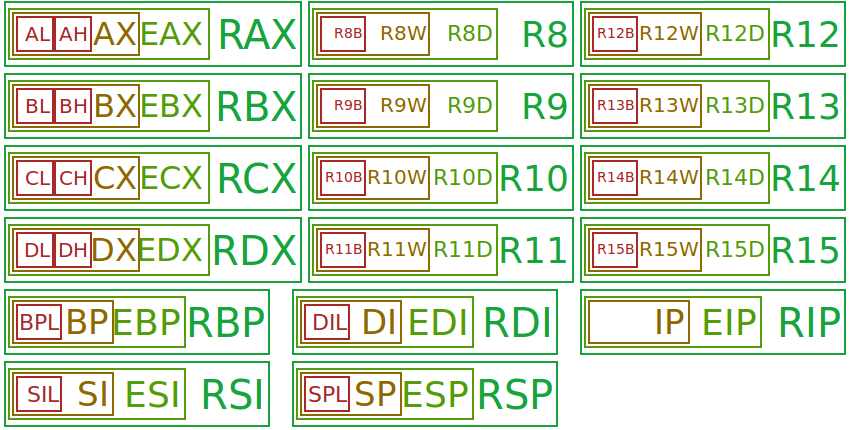
\includegraphics[width=\textwidth]{../asm/x86-gprs}
\imagecredit{Figure: Immae via Wikipedia}
\end{frame}


\subsection{authoritative source}
\begin{frame}{authoriative source (1)}
    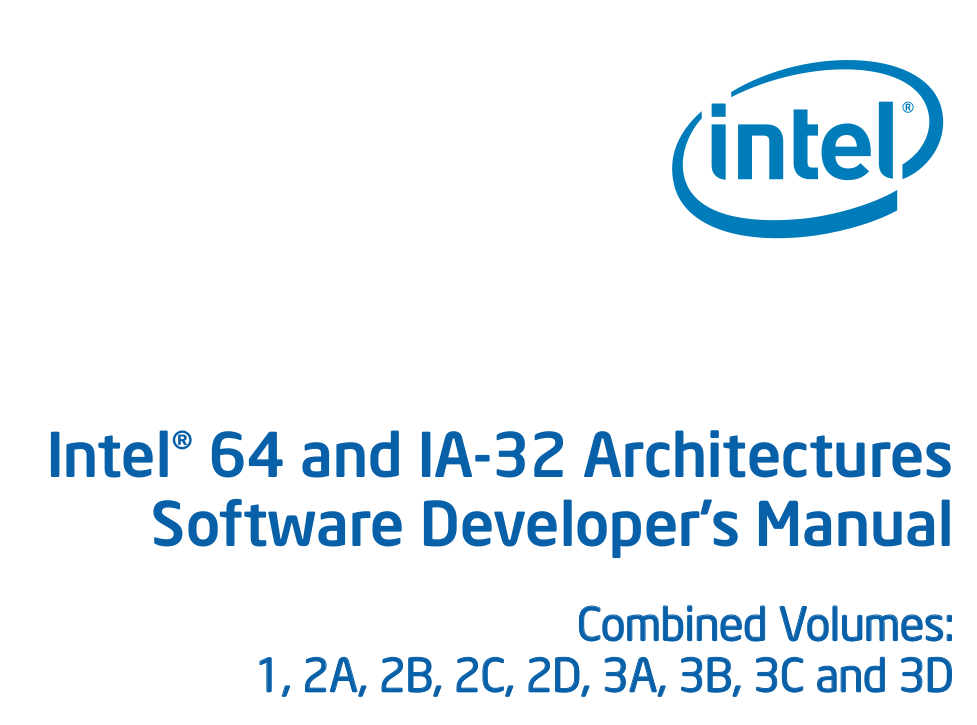
\includegraphics[height=.8\textheight]{../asm/manual-screenshot}
\end{frame}

\begin{frame}{authoriative source (2)}
    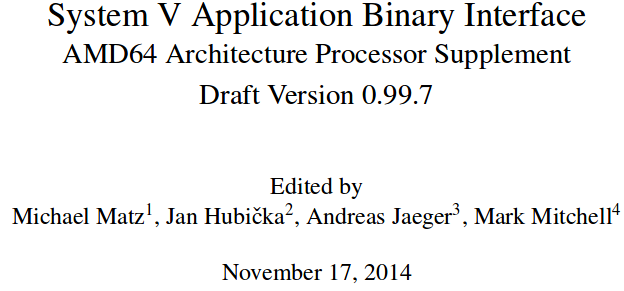
\includegraphics[height=.8\textheight]{../asm/abi-cover}
\end{frame}



\subsection{alt exercise}
\begin{frame}[fragile,label=asmQ]{question}
\begin{lstlisting}[language=myasm,style=small]
pushq $0x1
pushq $0x2
addq $0x3, 8(%rsp)
popq %rax
popq %rbx
\end{lstlisting}

What is value of {\tt \%rax} and {\tt \%rbx} after this?
\vspace{1ex}
\begin{tabular}{ll}
    a.& {\tt \%rax} = {\tt 0x2}, {\tt \%rbx} = {\tt 0x4} \\
    b.& {\tt \%rax} = {\tt 0x5}, {\tt \%rbx} = {\tt 0x1} \\
    c.& {\tt \%rax} = {\tt 0x2}, {\tt \%rbx} = {\tt 0x1} \\
    d.& the snippet has invalid syntax or will crash \\
    e.&  more information is needed \\
    f.& something else? \\
\end{tabular}
\end{frame}




\end{document}

